Time Response is sum of two responses: the natural response and the forced (kamel) response. \textit{natural response} is response of system to dirac delta on the other hand, \textit{forced response} is the response of system from applying an external force. To understand it in qualitatively manner remember what you know about a differential equation.
%\nicefrac{at}{2}
\subsection{Formulas}
\begin{minipage}{0.4\linewidth}
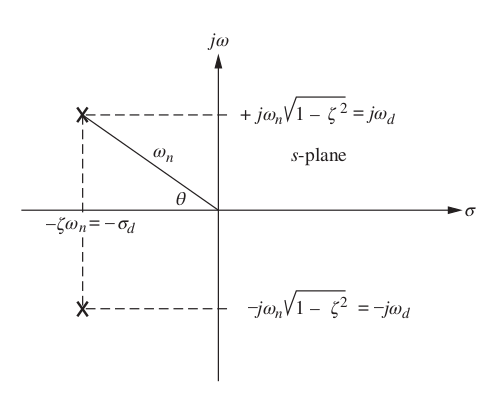
\includegraphics[width=0.8\columnwidth]{Resources/keesy.png}
\captionsetup{width=0.8\textwidth}
\centering
\end{minipage}
\begin{minipage}{0.6\linewidth}
$$ C(s) = \frac{\omega_n^2}{s^2+2 \sigma s + \omega_n^2} ~~ , ~~ c(t) = 1 - e^{ - \sigma t} \Big (cos(\omega_d t) + \frac{\sigma}{\omega_d} sin(\omega_d t) \Big)$$ 
$$ \zeta = \frac{\sigma}{\omega_n} ~~ , ~~ cos \theta = \zeta $$
$$ T_P = \frac{\pi}{\omega_d} ~~ , ~~ T_s = \frac{4}{\sigma}$$~
%$$ \%OS = \frac{c_{max}-c_{final}}{c_{final}} \times 100 ~~ , ~~ \%OS = \big  {e^{\mathlarger {-\sigma T_P}}} \times 100 $$
$$ \%OS = \frac{c_{max}-c_{final}}{c_{final}} \times 100 ~~ , ~~ \%OS = \big  e^{-\sigma T_P} \times 100 $$
\end{minipage}
~\\
%\scalebox{1.5}{\sfrac{3}{2}}
